\documentclass{article}

\usepackage[final,nonatbib]{neurips_2023}

\usepackage[utf8]{inputenc}
\usepackage[T1]{fontenc}
\usepackage{hyperref}
\usepackage{url}
\usepackage{booktabs}
\usepackage{amsfonts}
\usepackage{nicefrac}
\usepackage{microtype}
\usepackage{xcolor}

\usepackage{graphicx}
\usepackage{caption}
\usepackage{subcaption}


\title{LOLCATS: Leveraging Obscure Lexical Conventions And Tenuous Synonyms in computer science research}


\author{%
  Kyle Roth \\
  DIRO \\
  Université de Montréal \\
  Montréal, QC, Canada \\
  \texttt{kyle.roth@umontreal.ca} \\
  \And
  Georges Bélanger\thanks{An especially cool guy.} \\
  Affiliation \\
  Address \\
  \texttt{email} \\
  \And
  Alex Fulleringer\thanks{An especially cool guy.} \\
  Concordia University \\
  Montréal, QC, Canada \\
  \texttt{alexfulleringer@gmail.com} \\
}


\begin{document}


\maketitle


\begin{abstract}
  We did some stuff!
\end{abstract}


\section{Introduction}


We used the ART paper~\cite{paranjape2023art}.


\section{Background}


\section{Methodology}
%- provide tools that are analogous to long term memory in humans

Our goal was to create a modified ART framework that allows for an LLM to read from, write to, and organize a form of long-term memory, without actually retraining model weights.
This would allow for the model to dynamically access previously stored information, as well as update its local repository with valuable data as it reads through prompts.
Given the finite context window of any LLM, ensuring that only relevant data is retrieved would be a crucial requirement of this system.
With these goals and constraints in mind, we chose a Python dictionary as the underlying data structure for persisting information.
A dictionary naturally organizes data into key-value pairs, which would naturally allow for organization and efficient retrieval based on the LLM selecting only relevant keys.
The LLM would load the information stored at keys it finds relevant to its current task, and organize the information it stores by choosing an appropriate key.

In the context of ART, this translates into the creation of three tools to accomplish our envisioned task. Firstly, we define [list_keys], a tool that takes no inputs and returns a string containing all the keys in the dictionary.
Next we define [write], this tool requires a key-value pair and writes the pair into the dictionary, updating the value stored under the key if it is already present.
Finally, we define [read], a tool that takes a key as input and returns the information stored at that key in the dictionary.
Currently the tools save the dictionary to, and read it from, storage to ensure the long term stability of the data.

We demonstrate our tools by performing a summarization task on journal articles taken from DATASET HERE.
As is standard with ART prompts, demonstrations of the task are prepended to the prompt to provide the LLM an example of how to handle the task \cite{paranjape2023art}.
Each article is split into multiple chunks that are fed one at a time into the modified ART framework, with the network choosing how to organize and persist data for later perusal.
At the end of each article, each entry in the dictionary is then fed back into the LLM and a complete summary is generated. Experiments, results, and their analysis are discussed below.

\section{Experiments}


To effectively judge the usefulness of our method, we chose to evaluate on the abstractive summarization task. Unlike extractive summarization, in this task the summary is expected to be a concise representation that effectively communicates the key ideas in the text, rather than a composition of important phrases in the text. This is more like how humans generally summarize texts, and provides a stronger challenge for our method. We evaluated our method on the arXiv abstractive summarization dataset~\cite{cohan-etal-2018-discourse}. Texts in this dataset

\begin{figure}[h]
  \centering
  \begin{subfigure}{0.45\textwidth}
    \centering
    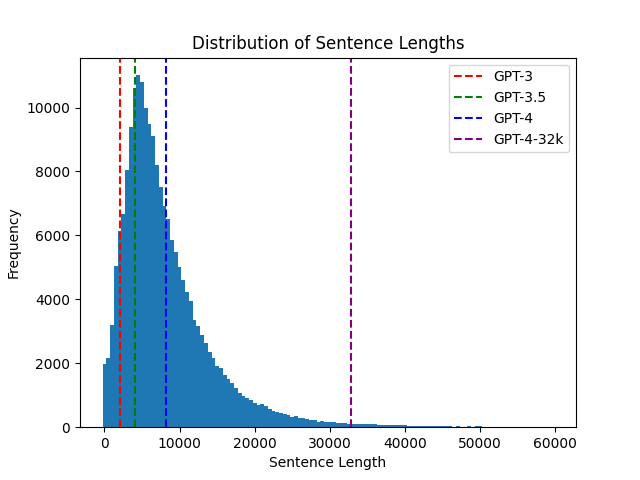
\includegraphics[width=\linewidth]{images/length_hist_train.png}
    \caption{Distribution of sentence lengths in the train set, by number of tokens. The sentence lengths have mean 8630.2, median 6883.0, minimum 0, and maximum 329071 (not visible).}\label{fig:train-hist}
  \end{subfigure}
  \hfill
  \begin{subfigure}{0.45\textwidth}
    \centering
    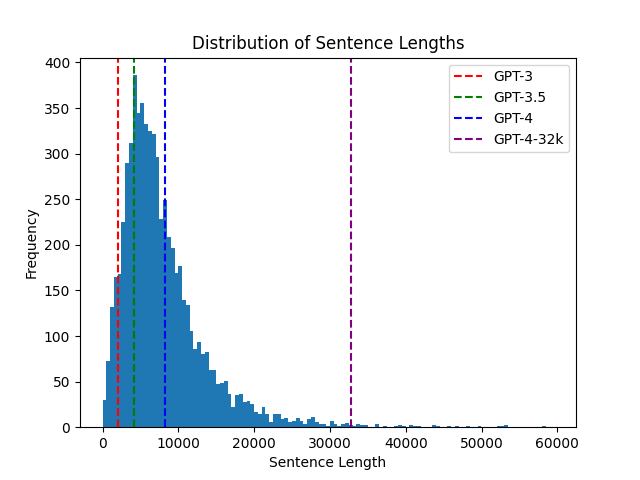
\includegraphics[width=\linewidth]{images/length_hist_validation.png}
    \caption{Distribution of sentence lengths in the validation set, by number of tokens. The sentence lengths have mean 8208.3, median 6871.5, minimum 244, and maximum 109442 (not visible).}\label{fig:val-hist}
  \end{subfigure}
  \caption{Distribution of sentence lengths in the train and validation sets.}\label{fig:length-hist}
\end{figure}


\section{Results}


\section{Conclusion}

- context window is limiting to ART framework
- future work in fine tuning a model instead of using a frozen one.
- lightweight models may be more appropriate
- Could be used for better conversational AI

In this project we have designed and implemented tools to be used by an LLM to organize and store relevant data for long-term/future use.
We encountered difficulties in providing enough context for the LLM to properly use the tools, but found some success with simplified run strategies.
Future research avenues could involve using newer, bigger, LLMs that have larger context windows allowing for more varied tool use samples to be passed as part of the prompt.
Otherwise, it may be desirable to fine tune smaller models specifically to use tools and address long standing issues with LLM capabilities.
To achieve the goal of an AGI system, it will be necessary for it to diversify its problem-solving across many contexts. 
Creating systems capable of learning to use tools may be an invaluable step along this path.

\bibliographystyle{neurips}
\bibliography{main}


\end{document}
